\scanpage{18}
% Pale pencil note in the top margin; the final 3.1 is written beneath the destination.
\begin{flushright}
\handwritten{\unsure{1.9.3|1.9.5}, \unsure{1.27|1.23}, 2.9 -- à reporter au \unsure{n\textsuperscript{o} 3}\unsure{?}}\\
\handwritten{3.1}
\end{flushright}

\(\mathbb{S}\)GA 4 VI

\uline{Sommaire}
\margin{\handwritten{\uline{\unsure{pp|pv}}}}

1. Conditions de finitude pour les objets et flêches d'un topos.\margin{\handwritten{-- 1 à 19}}

2. Conditions de finitude pour un topos.\margin{\handwritten{-- 20 à 37}}

3. Conditions de finitude pour un morphisme de topos. \deleted{\handwritten{Cas des \unsure{limites inductives}}}
\margin{\handwritten{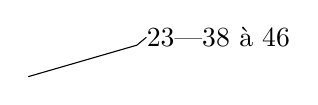
\begin{tikzpicture}[x=1cm,y=1cm,baseline=(r.base)]
\node[anchor=west,inner sep=0pt] (r) at (0,0) {\unsure{\deleted{2}3|3}8 à 46};
\draw (-1.5,-0.5)--(-0.12,-0.1)--(0,0);
\end{tikzpicture}}}

\deleted{4. Constructibilité.}
\inserted{\handwritten{4. Conditions de finitude pour un topos \inserted{obtenu par} recollement.}}\margin{\handwritten{-- 47 à 65}}

\deleted{5}\handwritten{6}. Catégories fibrées et $\underset{\handwritten{\longrightarrow}}{\mathrm{Lim}}$ (rappels).

\deleted{6}\handwritten{7}. Sites et topos fibrés.

\reversemarginpar
\margin{\handwritten{\begin{tikzpicture}[x=1cm,y=1cm,baseline=0pt]
\useasboundingbox (0,-0.1) rectangle (2.1,0.1);
\draw[overlay] (1.95,0.15) .. controls (1.95,-0.3) and (2.02,-0.55) .. (1.7,-0.62)
 .. controls (2.05,-0.7) and (1.85,-1.05) .. (2.0,-1.5);
\end{tikzpicture}}}
\normalmarginpar
\deleted{7}\handwritten{8}. Limites projectives de topos.

\deleted{8}\handwritten{\unsure{8|9}}. Cas des limites projectives filtrantes de topos cohérents par morphismes de transition cohérents: théorèmes de passage à la limite pour la cohomologie.

% Pencil relocation curve, its query and destination rule stay in the left margin.
\reversemarginpar
\margin{\handwritten{\begin{tikzpicture}[x=1cm,y=1cm,baseline=0pt]
\useasboundingbox (0,-0.15) rectangle (2.2,0.15);
\draw[overlay,->] (2.2,0) .. controls (0.05,1.25) and (0.05,2.9) .. (2.2,4.6);
\draw[overlay] (0.9,4.55)--(13.2,4.48);
\node[overlay] at (0.45,3.35) {?};
\end{tikzpicture}}}
\normalmarginpar
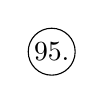
\begin{tikzpicture}[baseline=(n.base)]
\node[draw,circle,inner sep=1pt] (n) {\deleted{9}\handwritten{5}.};
\end{tikzpicture}
Cohomologie d'une limite inductive de fais\unsure{\deleted{x}c|\deleted{c}x}eaux sur un topos cohérent
% The right edge clips the last t; no following full stop is visible.

\reversemarginpar
\margin{\handwritten{
\begin{tikzpicture}[x=1cm,y=1cm]\draw[line width=2.5pt] (0,0)--(0.025,-0.28);\end{tikzpicture}}}
\normalmarginpar
\handwritten{10. Appendice (par P. Deligne). \deleted{Existence de point\unsure{s}} \unsure{\deleted{d'}Un|\deleted{d'Un}} topos cohérent \unsure{a} \inserted{suffisamment de points}\unsure{.}}

\deleted{NB \(\mathbb{B}\)ien sûr \handwritten{8} serait interchangeable avec le bloc \deleted{5}\handwritten{4} à \deleted{8}\handwritten{9}. Mais il me semble plus naturel de mettre dans deux numéros consécuti\unsure{\deleted{s}f|\deleted{f}s}s les deux facettes d\unsure{\deleted{y}u|\deleted{u}y} \unsure{\deleted{b}p|\deleted{p}b|\deleted{l}p|\deleted{p}l}assage à la limite en cohomologie. Bien sû\unsure{\deleted{t}r|\deleted{r}t}, le numéro \handwritten{8} sera réduit à une ou deux pages, le sorite des conditions de finitude étant déjà fait.}

\deleted{Le n\textsuperscript{o} 4 contiendra le sorite des groupes constructibles (au sens groupes finis ou non), des faisceaux de torsion, des notions de constructibilité pour les Modules et complexes de Modules, - y compris les faits spéciaux dans le cas localement noethérien. Je pense que je le rédigerai mais ne le garantis pas. On peut \deleted{à la rigu\unsure{e|r}} laisser t\deleted{l}\handwritten{o}mber le n\textsuperscript{o}4, ce sera alors moins beau bien sûr ...:}

\reversemarginpar
\margin{\handwritten{\begin{tikzpicture}[x=1cm,y=1cm,baseline=0pt]
\useasboundingbox (0,-0.1) rectangle (2.1,0.1);
\draw[overlay] (1.75,-0.2)--(2.0,-1.5);
\draw[overlay] (1.85,-0.2)--(2.13,-1.5);
\end{tikzpicture}}}
\normalmarginpar
\deleted{La rédaction qui suit des n\textsuperscript{o}s 1 à 3 est ào\unsure{\deleted{p}m|\deleted{m}p}plète, à cela près que je compte y ajouter encore quelques exemples (en particulier un topos localement algébrique non algébrique\handwritten{)}, \deleted{un morphisme non cohérent de topos cohérents).}
\inserted{\handwritten{et un topos ayant une famille génératrice formée d'objet cohérents, qui n'est pas localement algébrique}}}
% The long cancellation diagonals traverse all three lower paragraphs and the added lines; their chronological order is not asserted.
% archive sheet number: 17

